\section{STM32F4}
La Board si divide in due settori: Uno che contiene l'interfaccia di programmazione (si tratta di una scheda di progettazione), e si tratta di un altro microcontrollore removibile della ST che fa da interfaccia verso il computer (riceve il binario dal pc, e si interfaccia con il core con protocollo SVG o JTAG); L'altro settore invece contiene il SoC, che è proprio l'oggetto etichettato STM32F407VTGT6 (fig \ref{img:STM32F4}), mentre tutto ciò che c'è intorno consente all'utente di interfacciarsi con il SoC. 
I piedini presenti tra il SoC e la board sono condivisi tra più periferiche, quindi in fase di configurazione dobbiamo capire quale delle periferiche lo userà. Questi \textit{piedini} poi dovranno interagire con il mondo esterno, e ci viene in aiuto il \textit{jumper cable} che consente di collegare i pin della board con la periferica esterna.


\begin{figure}[h!]
    \centering
    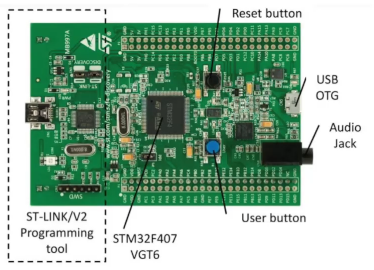
\includegraphics[width=.7\textwidth]{img/STM32F4.png}
    \caption{STM32F4}
    \label{img:STM32F4}
\end{figure}


Le periferiche illustrate sul \textit{reference manual} sono memory mapped, quindi raggiungibile mediante accessi in memoria. Per ogni periferica, in fase di configurazione si va a scrivere in alcuni registri in memoria. 

\subsection{CubeIDE}
L'IDE utilizzato al corso per la programmazione della scheda è STM32CubeIDE. \uppercase{è} importante selezionare la giusta board, perchè non si sta programmando un SoC nudo, ma una board, dove le periferiche sono mappate in maniera fissa su alcune piedinature del SoC. 
Una volta creato il progetto, ST fornisce un'interfaccia grafica per configurare i pin del MCU. 
Poichè i pin sono molto numerosi, sono raggruppati in \textit{porte}, enumerate con lettere. Ogni porta gestisce un determianto sottoinsieme di PIN. 
\\
\\
Onde evitare di configurare ogni periferica attraverso l'accesso in memoria e il modello di programmazione, i produttori di microcontrollori offrono un'astrazione delle periferiche denominate \textbf{HAL} (Hardware abstraction layer). Questi offrono un'interfaccia di programmazione astratta della periferica. 
